\chapter{Evaluation of Existing Applications}
\label{chp:3:EvalExisAppl}
After building the foundation by giving an overview about the related work on personalized mass email communication, this section will evaluate existing systems available in the market. 

\section{Application Categories and Their Relation with the Thesis}
\label{sec:3.1:SystCate}

There are three different application categories that are related with this thesis, and focus on email communication directly or indirectly. The following section will give a brief description of those categories, and their relation with this thesis:

\subsection{Customer Relationship Management (CRM)}
\label{subsec:3.1.1:Cust}
A \ac{CRM} application helps to manage customer relationships effectively, which is a topic studied both by academia and industry in recent years. Such applications play an important role in the marketing where organizations use more customer oriented instead of product or brand oriented marketing strategies. Therefore, each customer's economic value is different to the company, and organizations' customer relation strategies require adapting their customer offerings and communication strategy personalized according to individual customers \citep{Reinartz2004}. 
\vspace{1cm}

One of the reasons why this thesis considers evaluating \ac{CRM} applications is its communication aspect of a company with their clients. Another reason is, as it is mentioned at section 2.3, the adequate amount of personalization in emails is crucial on response rates, and people's increased daily interactions with the digital world make the true authentic personalization more rare. Achieving such a level of personalization requires getting to know each recipient very well by considering not only the recent conversation, but also earlier conversations. All the information that might be extracted from those conversations helps to build a relation with the respondents. Since a \ac{CRM} system aims to keep track of each customer history regarding a product or a brand, such a data store could be leveraged to add an adequate amount of personalized information to email conversation. 

\subsection{Help Desk}
\label{subsec:3.1.2:HelpDeskSoft}
Another application form that focuses on a company and its relation with their clients is help desk applications. Its main purpose is to provide information and support related to a company's products and services to their customers. As a part of knowledge acquisition, help desks support both sides of the communication in a way that while customers or end users find the knowledge they need, and the people who provide help by making the knowledge available and reusable \citep{Halverson2004}.
\vspace{1cm}

Reusing the existing knowledge requires to structure the captured knowledge. This is where it makes the relation with this thesis. Because, a help desk application provides a workflow where both parties develop a communication where a person who needs assistance describes his/her problem while people who provide help identify the problem by looking earlier cases or asking questions to clarify the initial question. This also requires the cooperation of assistants while providing help to a problem at which one person might have previous experience to guide other assistants. As a result, a help desk application is similar to a mass email communication where a researcher initiates an open ended questionnaire, extracting information from the coming replies, and organizes them according to the answers that he or she seeks for. In addition, respondents might also come up with some questions to clarify things, where existing answers can easily be reused. Having such a email conversation with large groups requires great effort from a researcher, so he might assign tasks to distribute the efforts to other researchers to deal with the large size of the group.


\subsection{Email Marketing}
\label{subsec:3.1.3:EmaiMarkt}
Organizations and marketers use email marketing for several reasons. Some of those purposes are brand and customer loyalty building, acquiring or converting customers, advertising the brand or the product, solicit sales or donation, communicating for promotional offers and even educational purposes. At the end, these approaches can be grouped under the following categories \cite{Eley2009}:

\begin{compactitem}
	\item \textbf{Educational Communication:} An educational message is given in the form of a newsletter, avoiding sale push, but it might still include some content encouraging recipients indirectly. For example, free monthly newsletter which contains tips about digital photography, and photography accessories used in the tips might be linked to an online shopping website. 
	\item \textbf{News and Updates:} To notify the customers about important updates or changes to a business. For instance, the release of a new product, changes on contact details or major changes on a company's website
	\item \textbf{Direct Sales Messages:} Emails sent by others consists of marketing ads, and clear messages on offers.
	\item \textbf{Housekeeping:} Emails such as subscription confirmation messages or welcome emails. These messages are often system generated automated messages. However, they can be used to promote a message as well like offering a discount code along with the registration confirmation email.
\end{compactitem}

Since these categories consist communication with a large group of people, this thesis also evaluates existing tools in the market for email marketing including their technical aspects.

\section{Methodology}
\label{sec:3.2:Meth}

The analysis examined two products from each of the categories that are \ac{CRM}, help desk, and email marketing. The selection of the products depends on several product comparison websites including Toptenreviews.com\footnote{http://\{email-marketing-software-review, crm-software-review\}.toptenreviews.com/ }, Softwareshortlist.com\footnote{http://www.softwareshortlist.com/crm/solutions/}, as well as the suggestions of Stanford HCI group members\footnote{http://hci.stanford.edu/people/}. In addition to those websites and suggestions, their demo or trial version availability was also considered, since some of the products required a fee before using them. After the products were shortlisted, the last filtering was done by getting their web traffic rankings from Compete.com\footnote{https://www.compete.com/}, Alexa\footnote{http://www.alexa.com/}, and Google Trends\footnote{http://www.google.com/trends/}. Finally, trial accounts of those applications were created, and a scenario was simulated to get the full insight from them. 

\section{Results}
\label{sec:3.3:Resul}
Evaluation of the products will be done according to their category. A brief description of the products will be presented. This description will mainly focus on the features, which are related to support email communication as explained in section~\ref{sec:3.1:SystCate}. After that each category will be concluded with a comparison matrix of the selected products.

\subsection{CRM Applications}
\label{subsec:3.3.1:CRMAppl}

SugarCRM and Highrise are the two \ac{CRM} applications that are analyzed in this thesis. Table~\ref{tab:comp_matr_crm} shows a summary of their features, and the following paragraphs give a more in-depth exploration for these products.

\clearpage

\begin{table}[H]
\begin{center}
	%\renewcommand{\arraystretch}{2}
	%\tiny
	%\setlength{\tabcolsep}{5pt}
	\caption[Comparison Matrix for CRM Applications]{Comparison Matrix for CRM Applications} \label{tab:comp_matr_crm}
    \begin{tabular}{ | p{3cm} | p{5cm} | p{5cm} | }
	\hline
	& \textbf{SugarCRM} & \textbf{Highrise} \\ \hline
	\textbf{Versions} & On-premise and SaaS & SaaS \\ \hline
	\textbf{Pricing} & \$35 -- \$100 user/month, and free community edition & \$24 -- \$99/month, and a free plan with limitations \\ \hline
	\textbf{Task Management} & Calendar based, no additional view & Individual module \\ \hline
	\textbf{Syncronization} & Plugins are available for Outlook, Lotus Notes & Require additional module installation \\ \hline
	\textbf{Email Client} & Build in, allowing email marketing with variable insertions & No \\ \hline
	\textbf{Contact Importing} & Via forwarding emails or plugins for Outlook, Lotus Notes & Outlook, Excel, vCard, or via forwarding emails \\ \hline
	\textbf{Mobile Support} & Yes & No \\ \hline
	\textbf{Analytics} & Marketing Analytics, sales forecasting and trends & No \\ \hline
    \end{tabular}
\end{center}
\end{table}

\paragraph{SugarCRM}
SugerCRM comes in three different deployment versions. These are on-premise, \ac{SaaS}, and the free community edition. It has a clean \ac{UI} with a single navigation menu. Its calendar view can be synchronized with Outlook's calendar or any platform, which supports iCalendar\footnote{iCalendar is the calendar data exchange stanard (RFC 5545) having file extension of .ics, and it allows sending meeting requests or tasks via email.}. It provides email management right in the application, and integrates with several platforms like Outlook and Gmail or an \ac{IMAP} based email server. Users can archive emails in the SugarCRM by adding a unique email address into TO, \ac{CC}, or \ac{BCC} fields. This address can also be used to link email recipients information including email attachments with SugarCRM by simply forwarding the emails, therefore it removes the additional effort to import them into SugarCRM and reduces dependency on a platform. SugarCRM also comes with a build in email client. Even though, its inbox view only provides basic functionalities, its email creation view goes a little further to support email marketing by providing dynamic variables that can be embed into an email's content, and can be replaced with actual values available in SugarCRM. For example, a variable for first name will be replaced by contact's actual first name while email is being sent (See figure~\ref{fig:SugarCRM-Create_Email}). 
\vspace{1cm}

\begin{figure}[htbp]
	\centering
	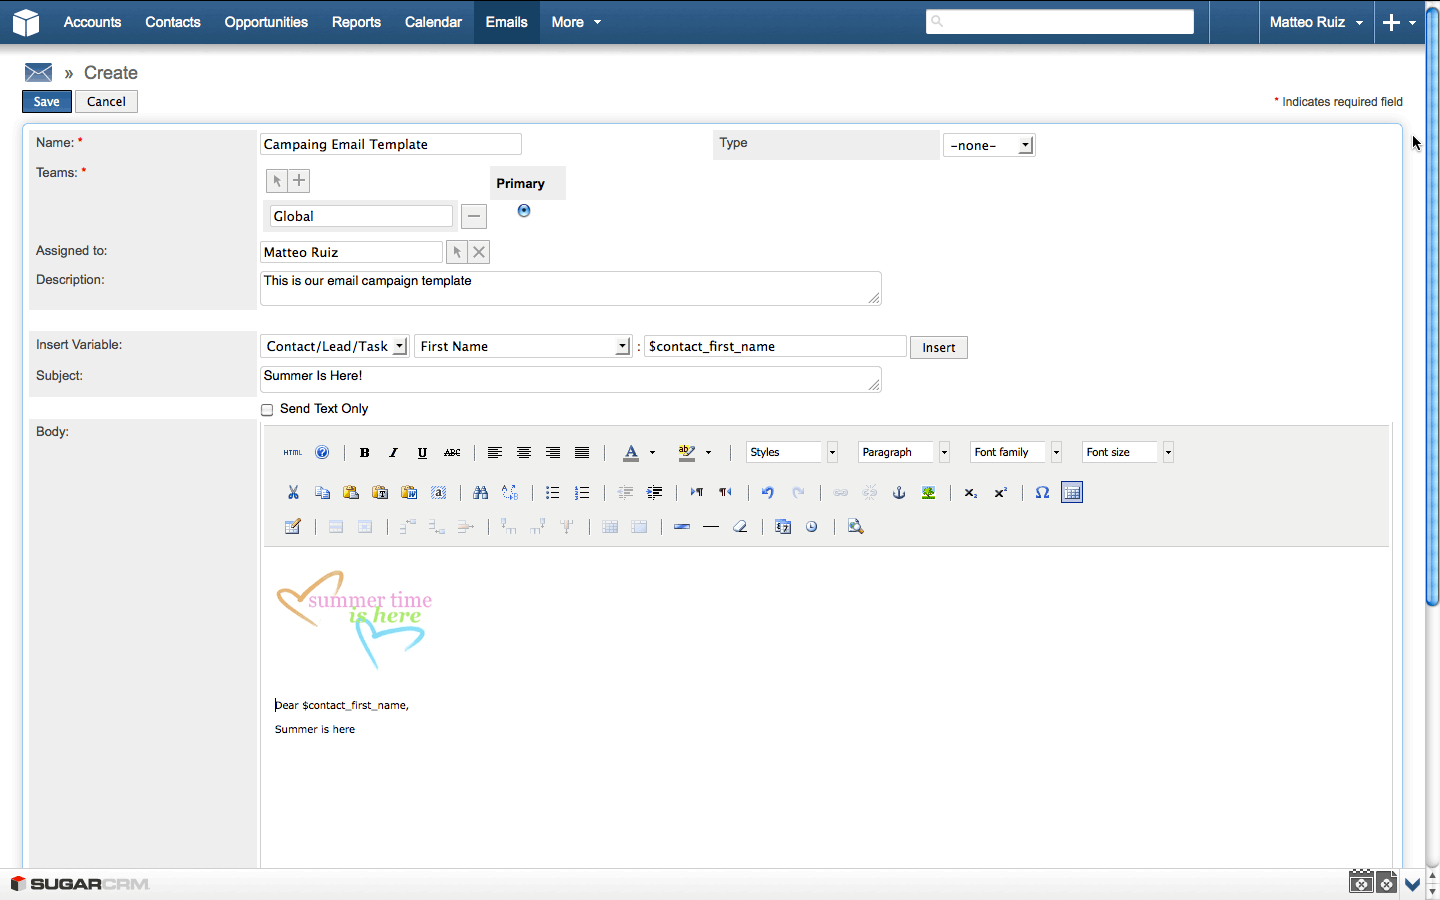
\includegraphics[width=1.00\textwidth]{imgs/SugarCRM-Create_Email.png}
	\caption[SugarCRM Email Composer with Embeded Variables]{SugarCRM Email Composer with Embeded Variables \citep{SugarCRMInc.2013}}
	\label{fig:SugarCRM-Create_Email}
\end{figure}

Initiated email marketing can be monitored to track response rates, generated leads, and unsubscribed contacts. Marketing target lists also can be imported from third-party lists. SugarCRM also let users save an email as a \ac{HTML} template to use it again within an email composer. Finally, it offers a mobile version to allow accessing most of the application features on smartphones and tablet devices \citep{SugarCRMInc.2013}.

\paragraph{Highrise}
Another \ac{SaaS} is Highrise\footnote{http://highrisehq.com/} offering several purchasing plans with 30 days trial period. It has a simple \ac{UI} like SugarCRM, but also provides quick access buttons to add a task or a contact. Task management differentiates it from SugarCRM since there is no calendar view, but a task view in Highrise. These tasks can be synchronized with iCalendar as well. In addition, users can create tasks from emails by using one of the unique email addresses for several time slots provided by Highrise, and adding them into \ac{BCC}, \ac{CC}, or simply forwarding an existing email creates a task in Highrise. Contact information can be imported from Outlook or by uploading a vCard\footnote{vCard is a file format standard for exchanging business contact information.} file. It provides all the basic contact information fields including the social accounts, however it does not offer custom field creation on those profiles. An email, including its attachments, can also be linked to a contact profile by simply forwarding it to the provided unique email address. If a user does not exist in Highrise when an email from him/her forwarded to link, a contact profile is created using available information in that email. Adding tags to the contact profiles also makes it easier to organize contacts and browsing within them. Highrise does not offer any email composer to do email marketing as in SugarCRM. Therefore, users will depend on another product to do simple campaigns. The provided activity view helps users to keep track of their own or other users' recent actions within Highrise. Lastly, it offers options to customize the look and feel of the application by provided color schemes \citep{37signals2013}.

\subsection{Help Desk Applications}
\label{subsec:3.3.2:HelpDeskAppl}

The two help desk applications investigated in this thesis are Zendesk and Kayako. Table~\ref{tab:comp_matr_help} provides a comparison matrix of their features, and the details are described in the following paragraphs.

\clearpage

\begin{table}[H]
\begin{center}
	%\renewcommand{\arraystretch}{2}
	%\tiny
	%\setlength{\tabcolsep}{5pt}
	\caption[Comparison Matrix for Help Desk Applications]{Comparison Matrix for Help Desk Applications} \label{tab:comp_matr_help}
    \begin{tabular}{ | p{3cm} | p{5cm} | p{5cm} | }
	\hline
	& \textbf{Zendesk} & \textbf{Kayako} \\ \hline
	\textbf{Versions} & SaaS & Software and SaaS \\ \hline
	\textbf{Pricing} & \$24 -- \$119 agent/month, and free trial & \$29 -- \$49 user/month, and free trial \\ \hline
	\textbf{Channels} & Website, email, phone, and social platforms & Website, email, and only Fusion version supports phone \\ \hline
	\textbf{Macros} & Yes, basic & Yes, advanced \\ \hline
	\textbf{Ticket Management} & Groups and tags & Types, statuses, priorities, and tags \\ \hline
	\textbf{Mobile Support} & Yes & No \\ \hline
	\textbf{Analytics} & Yes & Yes \\ \hline
    \end{tabular}
\end{center}
\end{table}

\paragraph{Zendesk}
Cloud-based customer service software Zendesk \footnote{http://www.zendesk.com} provides a nice and clean \ac{UI}. Zendesk has more than 30,000 businesses from a wide variety of industries. Zendesk offers one-on-one support via many different communication channels including website, email, phone, and social platforms like Facebook and Twitter. Hence, support requests coming from those platforms can be turned in to a support ticket. Those support tickets can be grouped under categories, and further classification can be done via tags for each ticket. Those feature also help to find related archived resolved tickets, so they can be reused for new tickets. Thanks to the automated process coming with macros a combination of actions can be done with one click like setting status, priority, type of a ticket, and assign it to another person with a predefined comment for the ticket. A ticket can be merged with another one, or copied to the forum to make it available to the public, which helps to create a knowledge base. Customer ticket history and basic personal information are kept in the system. However, it does not support to add additional fields to customers' profiles. In addition to the desktop version, Zendesk has a mobile version for smartphones and tablet devices. Therefore, support teams have no dependency on a device. Lastly, provided analytics view by reports give an overview of customer satisfaction and performance of the support team \citep{Zendesk2013,Zendesk2013a}.

\paragraph{Kayako}
Kayako's\footnote{http://www.kayako.com/} complete solution for customer support is named as Kayako Fusion. It comes as software and \ac{SaaS}. Comparing with Zendesk, its \ac{UI} seems more complicated. Kayako got more than 30,000 clients within ten years. Kayako does not have social platforms integration like Zendesk, therefore support tickets are generated over website, email, and phone. Tickets can have customized types, statuses, priorities, and tags. Similar to Zendesk, it also supports macros to assign tickets into a department, owner, type, priority, and provide canned responses for tickets with a click. Kayako also keeps basic information of customers, if they are registered to the system. Registered customers can also support to build a knowledge base in a forum-like environment by contributing others questions along with the support team. Kayako does not have any native app for mobile platforms like Zendesk. Finally, it has a analytics view to keep track of ticket reports, measuring customer satisfaction and support team performance \citep{KayakoInc.2013,KayakoInc.2013a}.

\clearpage

\subsection{Email Marketing Applications}
\label{subsec:3.3.3:EmaiMarktAppl}

MailChimp and Constant Contact are the selected two email marketing applications to analyze in this thesis. Table~\ref{tab:comp_matr_emai} shows their features side by side to give an overview. The details are provided in the upcoming paragraphs.

\begin{table}[H]
\begin{center}
	%\renewcommand{\arraystretch}{2}
	%\tiny
	%\setlength{\tabcolsep}{5pt}
	\caption[Comparison Matrix for Email Marketing Applications]{Comparison Matrix for Email Marketing Applications} \label{tab:comp_matr_emai}
    \begin{tabular}{ | p{3cm} | p{5cm} | p{5cm} | }
	\hline
	& \textbf{MailChimp} & \textbf{Constant Contact} \\ \hline
	\textbf{Versions} & SaaS & SaaS \\ \hline
	\textbf{Pricing} & \$10/month with max 500 subscribers -- \$240/month with max 50,000 subscribers. Pay as you go available & \$15/month with max 500 subscribers -- \$75/month with max 10,000 subscribers. \\ \hline
	\textbf{Template Editor} & Drag and drop including advanced photo editor & Drag and drop including basic photo editor \\ \hline
	\textbf{Recipients List} & Conditional filtering & Grouping \\ \hline
	\textbf{Variable Support} & Yes, advanced & No \\ \hline
	\textbf{Permissions} & Admin, manager, author, and viewer account types & None \\ \hline
	\textbf{Mobile Support} & Yes & No \\ \hline
	\textbf{Analytics} & Yes & Yes \\ \hline
    \end{tabular}
\end{center}
\end{table}

\paragraph{MailChimp}
MailChimp\footnote{http://mailchimp.com/} comes as \ac{SaaS}, and offers fixed cost monthly plans or pay as you go plan. Along with its intuitive \ac{UI}, it offers a drag and drop functionality on the email content creation. It supports email marketing processes starting from designing the sign up form, so users can add all the desired fields, and apply brandings to it. The recipients' list can be filtered out with several conditions like campaign name, location, or ratings assigned by application's user. There are different levels of access privileges to MailChimp. Hence, a person who has an "Admin" account can grant permissions different type of permissions allowing different access levels to MailChimp. This allows a separation of tasks in mail marketing. For instance, while managers manage recipients list, an author team can focus on emails' content and design \citep{TheRocketScienceGroupLLC2013}. To design email content, users can pick one of the available templates provided by MailChimp or create their own \ac{HTML} templates with its drag and drop editor (See figure~\ref{fig:MailChimp-DragAndDropEditor}).
\vspace{1cm}

\begin{figure}[H]
	\centering
	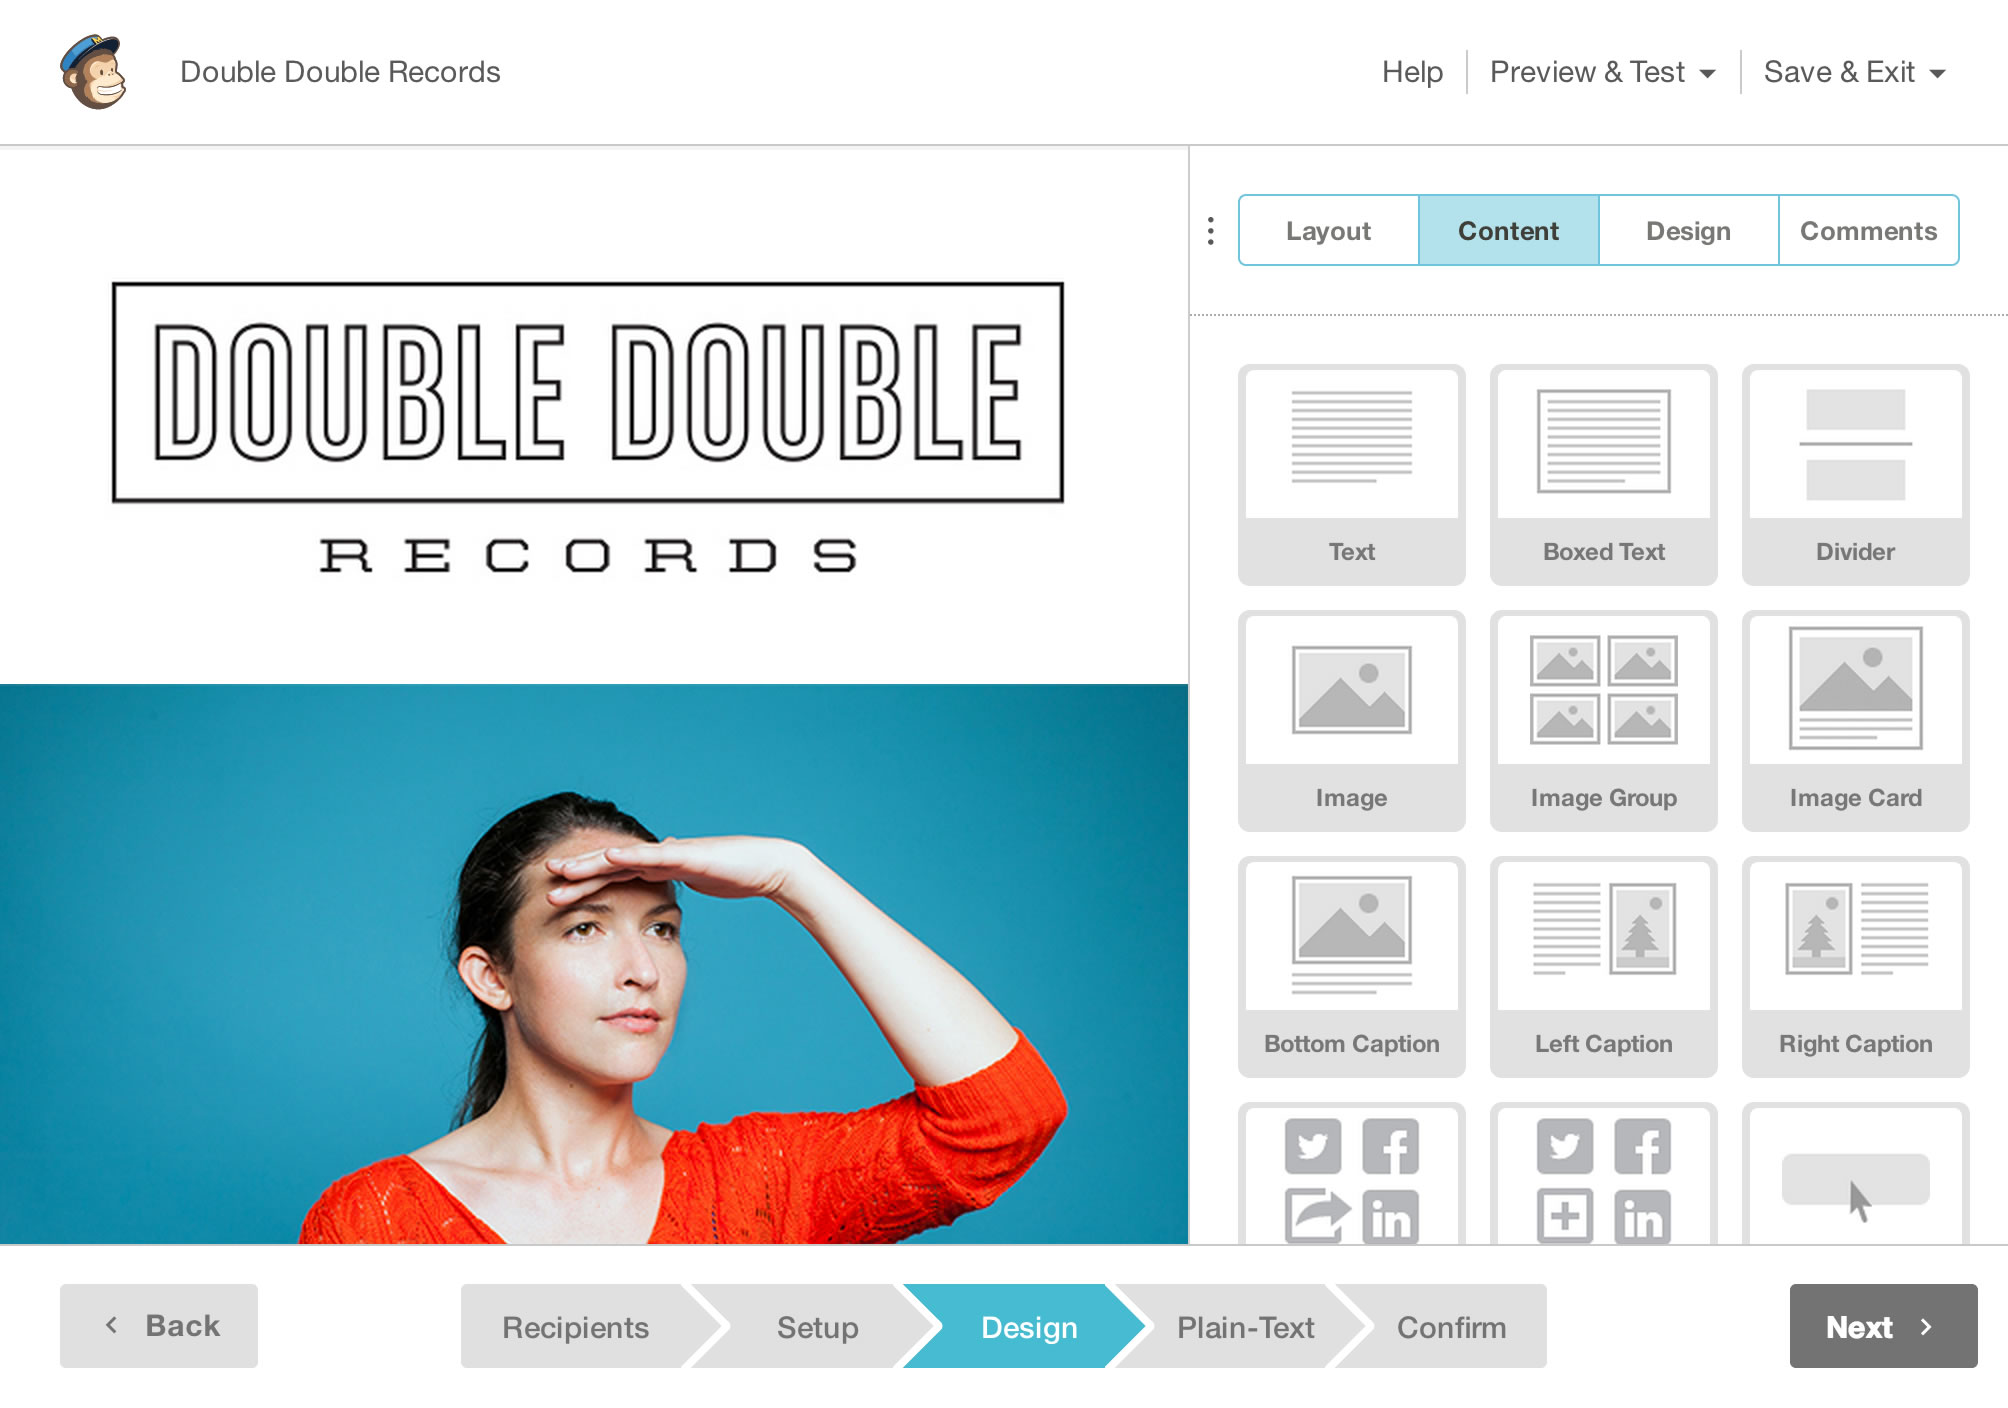
\includegraphics[width=1.00\textwidth]{imgs/MailChimp-DragAndDropEditor.jpg}
	\caption[MailChimp Drag and Drop Content Editor]{MailChimp Drag and Drop Content Editor \citep{TheRocketScienceGroupLLC2013a}}
	\label{fig:MailChimp-DragAndDropEditor}
\end{figure}

The template editor also provides a photo editor, and authors can add comments to give feedback on the content and design of the templates. Created templates can be previewed as if they are viewed in a software or an online email client, or even a mobile browser \citep{TheRocketScienceGroupLLC2013a}. As in SugarCRM, MailChimp allows you to use dynamic variables, called merge tags, in the email content. Therefore, send out emails can be personalized with information specific to the recipients. However, it provides more different type of dynamic variables than SugarCRM, and it is possible to add a conditional logic to them. For example, in listing~\ref{lst:MailChimCondMergTags}, a custom discount message will be shown in the email depending on the US state of recipients.
\vspace{1cm}

\lstset {
 basicstyle=\footnotesize,
 frame=shadowbox,
 rulesepcolor=\color{black},
 showspaces=false,showtabs=false,tabsize=4,
 numberstyle=\tiny,
 captionpos=b,
 xleftmargin=0.7cm, xrightmargin=0.5cm,
 lineskip=-0.1em,
 abovecaptionskip=1\baselineskip
}

\begin{lstlisting}[language=XML, caption={[MailChimp's Conditional Merge Tags]MailChimp's Conditional Merge Tags \citep{TheRocketScienceGroupLLC2013b}}, label={lst:MailChimCondMergTags}]
	*|IF:STATE=CA|*
		Save 20% on surf boards!
	*|END:IF|* 
	*|IF:STATE=GA|*
		Save 20% on Mountain Bikes!
	*|END:IF|* 
	*|IF:STATE=FL|*
		Save 40% on water skis!
	*|END:IF|* 
	*|IF:STATE=CO|*
		Save 50% on ski gear
	*|END:IF|*
\end{lstlisting}

MailChimp offers auto-response based on a triggering event. These events can be a link clicked in the email, being on a specific date like birthday of a contact, or scheduled dates. Finally, there exists an analytics dashboard where users can track the amount of opened emails, or the click rates of the links in the emails \citep{TheRocketScienceGroupLLC2013c,TheRocketScienceGroupLLC2013d,TheRocketScienceGroupLLC2013e}.

\paragraph{Constant Contact}
Another email marketing \ac{SaaS} is Constant Contact Email Marketing\footnote{http://www.constantcontact.com/email-marketing}, whose purchase plan depends on the amount of contacts you have, but there is a free 60 days trial period as well. It offers drag and drop content creation like MailChimp with a clean \ac{UI}. It has quite many templates to pick and start customizing it. However, users can embed sign up forms into websites or Facebook. Recipients list can be imported from several sources including Excel, Outlook, and Gmail. In addition, recipients can be grouped under sublists which can also be merged into each other easily. An option is available to remove duplicate contacts from the lists or delete recipients who unsubscribed from the list. Users can track opens, clicks, forwards, and social platform shares of their email campaign. On the other hand, it does not offer any sophisticated email variables to be replaced by actual content from the application \citep{ConstantContactInc.2013,ConstantContactInc.2013a,ConstantContactInc.2011}. 

\clearpage

\section{Conclusion}
\label{sec:3.3:Conc}
In conclusion, aforementioned applications in three different categories support email communication in several ways:

\begin{compactitem}
	\item Contact User profiles kept in \ac{CRM} applications can help a researcher to get to know their respondents better and to identify basic attributes like name, gender, address, and phone numbers. However, those fields were limited with fixed fields in those applications.
	\item Importing contacts information from other popular software, e.g. Outlook, can ease the time to create recipient lists for email communication. Again as SugarCRM and Highrise supports, importing an email into the system by just forwarding it to a specific email address can make researchers life easier in the same way. Providing such flexibility will reduce the dependency on a platform, therefore while researchers continue to use their email clients that they are familiar with, they can switch to another platform when it is necessary.
	\item Both \ac{CRM} applications provides a module to create tasks, so this can be helpful to remind researchers what is the next high priority thing to do about an email campaign. This can be a task showing what is next to do in an email campaign initiated by the researcher. For instance replaying the email in which the respondent has asked a clarifying question at our initial campaign.
	\item Both \ac{CRM} applications support archiving of emails by simply forwarding them to a provided unique email address, and linking those emails to the users' profile. This can be helpful to see important conversations happened with respondents earlier time, so it can provide content or an opinion about how to initiate upcoming conversations with those people. However, forwarding an email is an additional step, which requires additional effort and time.
	\item Reusability of earlier emails is important not to write them again. As we have seen, SugarCRM also allows saving emails as a template to reuse them again. However, there was no filtering mechanism or similar functionality, but just remembering the given name of the template to help users find the corresponding template to reuse.
	\item It is not always the case that a researcher initiate an email communication. It might be the case that a high amount of email can be dropped into the researchers inbox. For example, students attending a course may ask questions regarding their homework. In that scenario, the same question might be asked several times. Help desk applications provide a ticketing system for customer related issues, which is also applicable to the mentioned homework scenario. Therefore, existing email replies can be reused for further recipients.
	\item Both help desk applications support tagging or grouping of incoming emails, which can be helpful to identify conversations belonging to each other in a situation where a researcher initiated more than one campaign. However, there was no visual representation of the state of the communication of a support ticket, but just status labels like "resolved" or "assigned".
	\item Another feature of help desk software is a support ticket that can be shared or assign anyone by anyone from the support team. Hence, this will decrease the answering time of those tickets. This can be also useful in a mass email communication to share the responsibility to reply or extract information from incoming emails.
	\item The email marketing application MailChimp provides dynamic variables that users can add into email content and its variable will be replaced with actual values. Such a feature can be helpful in personalized mass email communication, where it is difficult to add recipient specific personalized information into emails. However, there was no attached information regarding those variables to show users in which state of the communication they are extracted, and again they were created separately in an additional view where users are away from the actual emails where they can extract information.
	\item MailChimp also provides different type of permissions to leverage in an email marketing task. For instance, while an author can create the email content, a viewer can just follow the reports to see what is the success rate of an initiated campaign. Such functionality can also be helpful in mass email communication, where some users can extract the information from emails, others can reply the emails.
	\item Both email marketing and helpdesk applications provide analytic reports to keep track of the success of a campaign or a support team. That is a useful function in a mass email communication as well to get a quick overview of the state of the communication.
\end{compactitem}

As mentioned above, there are many useful features that can be helpful to ease a mass email communication. However, there is no one specific application doing all the mentioned features, or doing them in a way to support their main purposes, which are \ac{CRM}, help desk, and email marketing.

\begin{comment}
As it is mentioned in~\ref{sec:2.3:PersEmai}, recipients intense daily interaction with digital devices make the true authentic personalization rare, and resulting low response rates. Therefore, it is important to have a platform where researchers can easily extract information, and leverage them again for the personalization of further email communication too.
\end{comment}

\vspace{1cm}

In the next section, an initial prototype will be introduced to support the workflow of a personalized mass email communication.

\begin{comment}
--> At the end, put the all the comparison tables together to the Appendix
--> These features are also helped us to add them into our app, decided by saying they all support so we can also support
--> HDesk provides reusibility of emails, CRM provides contact details to replace in email content
\end{comment}
